\chapter{Discussion}
\label{chap:discussion}
In this final chapter, the research results are discussed and contextualized with the research questions (see Chapter 3.1) and the idea that inspired this work: evaluating the feasibility of performing real-time Emotion-Recognition with a wearable device for a future affective BCI system. 

\section{Challenges towards real-time Emotion-Recognition}

When imagining users adopting a technology in the real life as a product, many functional and design aspects are rightfully expected. For example, the design of the device needs to be sleek and intuitive, and the flow of the application must be seamlessly integrated and well performing. This is clearly not the case for current Brain-Computer Interfaces, that are still in their infancy and far from mass adoption, especially for healthy users. Lin, Jung and Onton \cite{lin_toward_2015} reviewed methods that could greatly improve the quality of the user experience and finally open the way for affective \ac{BCI} to reach the consumer market. The core challenge of affective \ac{BCI}  is to create a plug-and-play \ac{BCI}  system with limited electrodes that can consistently perform accurate Emotion-Recognition regardless from the person that is using it. The other challenges consequently follow:
\begin{itemize}
\item 	Reduction and selection of electrodes: the number of electrodes must be relatively small, between 2 and 8, and strategically placed over the cortical areas delegated to the processing of emotions. They also should be soft dry electrodes and the system should be able to automatically recognize bad channels and excluding them from the processing.
\item 	Automatic artifacts cleaning: artefacts are one of the most impacting problems, and currently the most popular approaches for offline artifact cleaning are \ac{ICA}, that is not applicable to small sets of electrodes and too computationally expensive for online cleaning, and visual inspection. Alternative approaches might be achieved using regression to train algorithms in recognizing specific types of artifacts or features of the signal that indicate whether the quality is good or not and adjust it accordingly. Cleaning artifacts is also vital to the efficient use of as much data as possible. In the current study the artifacts removal strategy led to the exclusion of 10 participants and up to 25\% of the data of the remaining participants, a considerable cost considering the time and efforts needed to collect the data with an experimental protocol.
\item 	Features selection and reduction: selecting the most suitable features allows to reduce the computational cost by removing redundant and less meaningful features, and this is particularly correlated to the selection of electrodes as well. Lin et al. \cite{lin_toward_2015} through their extensive research over the years discovered that differential asymmetries are the most consistent type of features among subjects and sessions, reliable also for subject-independent classification. In more recent studies, Thammasan et al. \cite{thammasan_continuous_2016}, Keelawat et al \cite{keelawat_comparative_2021} and Avramidis et al. \cite{avramidis_multiscale_2021} , extracted \ac{EEG} features using fractal dimension algorithms instead of \ac{PSD}, obtaining significantly better performances in both subject-dependent and subject-independent classification. Another possibility is to use more complex models like \ac{CNN} \cite{keelawat_comparative_2021} to automatically extract features from the \ac{EEG} signal, losing the ease of interpretability of the model and the direct connection with the theoretical neuroscience.
\item 	Users training and calibration: a very time consuming and frustrating process is the calibration of \ac{BCI} systems for new users, especially if they have no experience of brain-controlled inputs. A system that can only classify emotions with a subject-dependent strategy is bound to train the users in reporting their emotions and then train a classifier with the collected data, all under the assumption that the resulting dataset is not too unbalanced. This of course is not feasible, and ultimately subject-independent classification should be the aim for real-time systems. However, this might not suffice, and even subject-independent classifiers might have to be tuned with short calibration sessions to adjust for each specific case, for example by selecting more susceptible features for a certain user that matches similar brain “signatures” from a group of users that the model has already been trained on. Zero-training strategies \cite{krauledat_towards_2008,jeong_hybrid_2021} have been object of study over the last decade and using spatial filters and transfer learning makes it possible to train a sub-optimal decoder and then use unsupervised learning to transform it into a user specific decoder. Of course, these solutions are still very experimental and use case specific, and further investigation is required.
\end{itemize}

The rest of the chapter will contextualize these challenges in the current study. Using a wearable EEG is a solution to the first problem, but also a constraint around which every other problem had to be worked around.

\section{Self-reported emotional labels}

Reporting emotions is a non-trivial task and could be subjectively difficult. From the feedback forms collected after the experiment, 7 subjects reported to have found difficulties in choosing the quadrant of the valence-arousal space, 8 subjects reported difficulties in assessing the emotional intensity (in both dimension) and 9 subjects reported difficulties in assessing the specific emotions. In addition, participants reported an average fatigue score of 2.47 ± 0.97 after the first half of the experiment and a fatigue score of 3.27 ± 0.86, on a scale from 1 to 5. Some emotions were reported to be missing from the simplified valence-arousal space, for example annoyance. Another missing emotion was “bittersweet”, that is commonly experienced in music listening yet difficult to report because of its composition of not-adjacent emotions (sadness, happiness) on the valence-arousal space. Continuous annotation of emotions has several advantages over discrete annotation, allowing a more granular reporting that consider emotional “oscillations” over the duration of a stimulus and more distributed labels across all classes that can favor the classification task.  It is a powerful tool for researchers to build affective datasets but heading towards a real product it will eventually be an obstacle as it requires an extra layer of training before the calibration. Discrete annotations are a simpler task that has virtually no impact on the recording phase and can be more easily integrated in a calibration tool, but seemingly yielding poorer performances compared with the continuous approach \cite{thammasan_continuous_2016}. An example to compromise the benefits of both approaches could be a subject-independent classifier trained using an offline dataset collected with continuous labelling, then discrete annotations collected by an online system would be used to integrate subject-specific differences during a calibration phase.

\section{Familiarity, liking and PANAS}

During the experiment, participants were asked to rate every song they listened to in terms of how much they liked the song referred to as “liking” and how much the song was familiar to them referred to as “familiarity, both on a scale from 1 to 5 where “3” represents neutrality. These scores could be used in a music recommending system to enhance the quality and relevancy of recommendations, however for the current research they were only used to assess the impact of the selected stimuli. The average “liking” score across all trials and all participants 3.32 ± 0.52, indicating that the selection has been in general positively perceived. Average “familiarity” score was 2.26 ± 0.53, quite below neutrality despite most of the songs being from internationally known artists. Having general low familiarity is positive for classification as emotional biases caused by memories can occur. Looking at Tables 1 and 2 in Chapter 5.1 it is also possible to observe that some of the participants with highest average “familiarity” are also among the worst classification scores, but the analysis was out of the scope of this research. Further investigation is needed regarding the correlations of “liking” and “familiarity” with the emotional dimensions of valence and arousal. Before each session, participants were also asked to fill a PANAS questionnaire. 

\begin{figure}[h!]
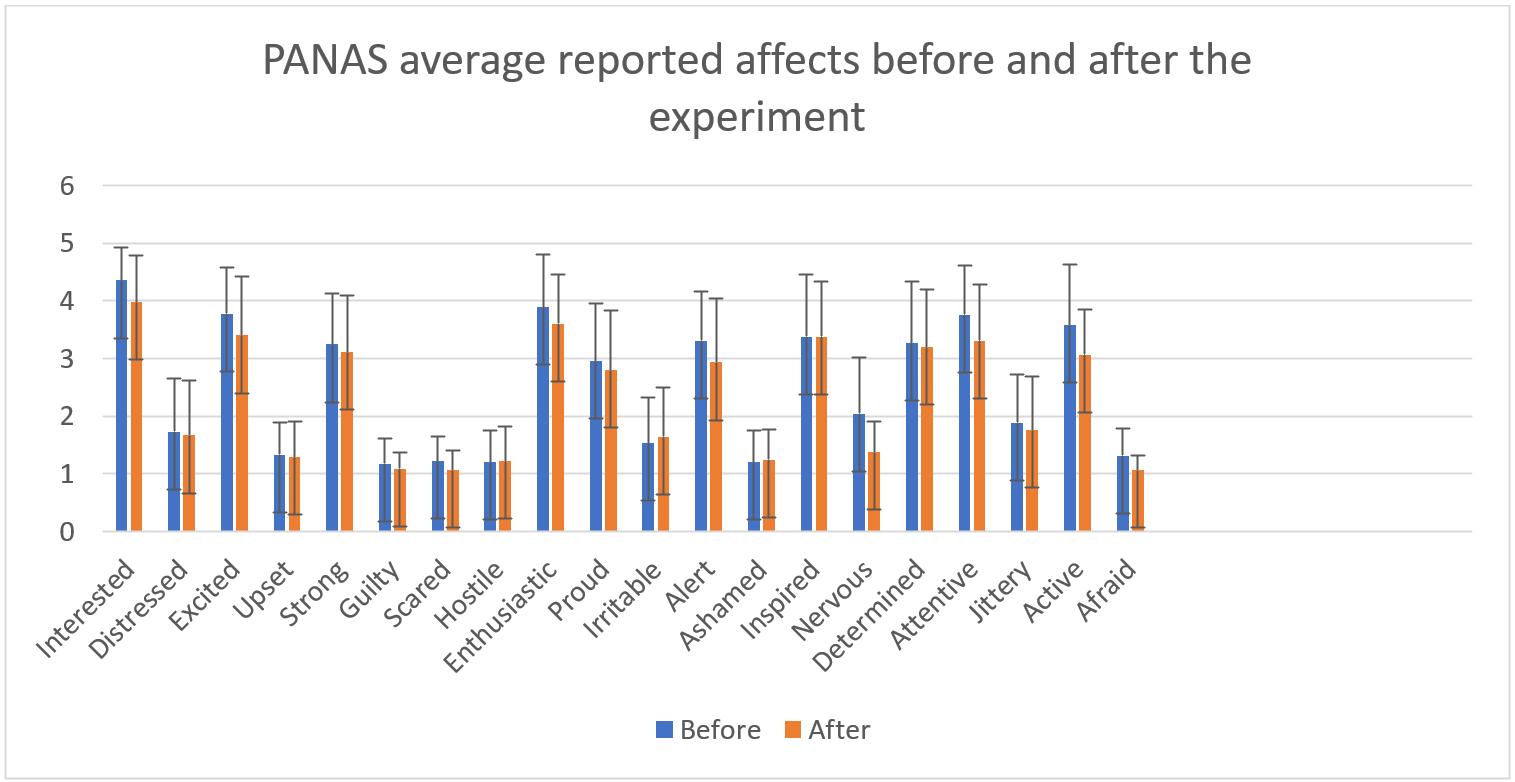
\includegraphics[width=12cm]{img/discussion/panas.png}
\centering
\caption{Average reported affects before and after the experimental session.} \label{fig:panas}
\end{figure}
Comparing the assessed affects before and after the experiment (Fig. \ref{fig:panas}), it is possible to observe that general interest, enthusiasm, and excitement of the participants decreased, which was expected considering that for the majority of the participants it was the first time participating in an EEG experiment. Attentiveness and activeness also significantly decreased, suggesting that the task proposed, and the length of the session were to some degree causing fatigue. Follow-up experiments can account for these effects by shortening the length of musical excerpts, reducing the number of conditions, or distributing the data collection from each participant over multiple sessions.

\section{Features selection and performances evaluation}

The proposed principal features based on previous findings on differential and rational asymmetries were the neuromarkers: \ac{AWI}, \ac{FMTI} and \ac{SASI}. The frequency-band specific features of the \ac{EEG} signal were extracted using the SignalProcessingToolbox proprietary library from myBrainTechnologies. Intermediary experiments using forward \ac{SFS} revealed a general trend in selecting the neuromarkers as most significant features, with some exceptions. \ac{PCA} was then used instead of \ac{SFS} as better performing subject-dependent features selection method to reduce the dimensionality of the features vector in lower computational time. It was not possible to directly compare the impact of using neuromarkers instead of frequency-band specific features, but the results were very promising for a subset of participants. The evaluation of model performances using \ac{MCC} score led to better understanding and correcting models who were over-fitting toward the majority classes because of uneven distributions of labels. It made possible to easily identify under-fitting models, however no solution was found to prevent it. Overall, \ac{MCC} score seems to be a more reliable score to describe the learning capabilities of the models, and it is better to compare with the most recent related studies instead of classification accuracy.

\section{From subject-dependent to subject-independent classification}

Clearly, subject-dependent classifiers are a sub-optimal solution for a real-time system and pose a threat to the usability by requiring full training sessions for new users. Besides, training a separated model for each user is not a long-term scalable solution. However, due to the subjective differences, subject-dependent remains the current preferred choice for Emotion-Recognition. Subject-independent strategy is only applicable to set of features that can represent the same emotional patterns for everyone, for example differential asymmetry seems to be very promising \cite{lin_toward_2015}, but also assumes that all the datasets used for training are as clean as possible to prevent the contamination of artefacts. In the current study it was not possible to obtain better than default-guessing for subject-independent classification. Some conditions are likely to hinder classification:

\begin{itemize}
\item 	Artifacts: Data might be too affected by artifacts, hindering any classification.
\item 	Features: Selected features might not be suitable for all subjects, or they might be suitable only for groups of subjects with similar “brain signature”.
\item 	Labels: Distribution of the classes can be highly uneven, and self-reported labels can be unreliable.
\item 	Electrodes: Two electrodes might not contain sufficient significant data; they can be misplaced or bad conducting.
\end{itemize}
The enormous performance difference among subjects in subject-dependent classifications suggests that improvements in the first three conditions are not only possible, but also necessary towards the creation of wearable affective \ac{BCI}s. If the low number of electrodes were the main impediment to classification, it would not have been possible for some participants to score more than 80\% classification accuracy. After reducing the variability created by these conditions and once subject-dependent classification will yield consistent performances among subjects, it will be possible to further develop a hybrid paradigm where a subject-independent classifier serves as sub-optimal basis for fast calibration of subject-dependent classifiers. Finally, if these goals are met, full subject-independent classification will be the next step towards affective \ac{BCI}s.
